\section{Optik}

\subsection{Principer}

\paragraph{Huvudplan och fokalplan}
Betrakta figur \ref{fig:optical_planes}.
\begin{figure}[!ht]
	\centering
	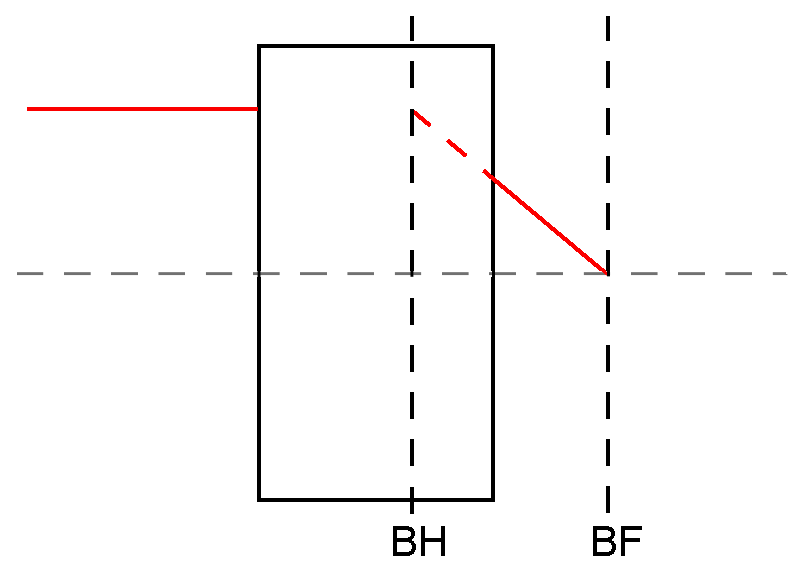
\includegraphics[scale=0.8]{./Images/optical_planes/optical_planes.eps}
	\caption{Illustration av bakra huvdudplan och fokalplan för ett godtyckligt optiskt system.}
	\label{fig:optical_planes}
\end{figure}

Lådan illustrerar ett optiskt system. Den röda strålen representerar strålgången. Det bakra fokalplanet, märkt BF, är planet där en parallell stråle skär den gråa centrallinjen och som är normalt på centrallinjen. Det bakra huvudplanet, märkt BG, är planet så att det optiska systemets verkan på strålan är ekvivalent med att all brytning sker i det planet, som illustrerat. Det fremre fokalplanet och huvudplanet fås på analogt sätt om man betraktar en stråle som kommer från höger.

\paragraph{Fokalavstånd}
Fokalavståndet till ett optisk system är avståndet från systemets bakre huvudplan till dets bakre fokalplan.

\paragraph{Konvexa och konkava linser}
En konvex linsa samlar parallela strålar, medan en konkav lins sprider parallella strålar.

\subsection{Ekvationer}

\paragraph{Reflektionslagen för plana speglar}
\begin{align*}
	s = -s'
\end{align*}
Alternativt, i kartesisk konvention:
\begin{align*}
	s = s'.
\end{align*}

\paragraph{Spegelekvationen för sfärisk spegel}
\begin{align*}
	\frac{1}{s} + \frac{1}{s'} = \frac{2}{R}
\end{align*}
Alternativt, i kartesisk konvention:
\begin{align*}
	-\frac{1}{s} + \frac{1}{s'} = \frac{2}{R}
\end{align*}
$R$ är spegelns krökningsradie.

\deriv

\paragraph{Brytning i sfäriska ytor}
\begin{align*}
	\frac{n_1}{s} + \frac{n_2}{s'} = \frac{n_2 - n_1}{R}
\end{align*}
Alternativ, i kartesisk konvention:
\begin{align*}
	-\frac{n_1}{s} + \frac{n_2}{s'} = \frac{n_2 - n_1}{R}.
\end{align*}

\deriv

\paragraph{Linsformeln för tunna linser}
\begin{align*}
	\frac{1}{s} + \frac{1}{s'} = \frac{1}{f}
\end{align*}

\deriv

\paragraph{Linsformeln för krökt lins}
\begin{align*}
	\frac{1}{s} + \frac{1}{s'} = \left(\frac{n_2}{n_1} - 1\right)\left(\frac{1}{R_1} - \frac{1}{R_2}\right)
\end{align*}